\documentclass[12pt]{article}
\usepackage{amsmath, amsthm, amssymb, amsfonts, graphicx}

\title{Exam II \\
\small Differential Equations \\
University of Massachusetts Lowell \\
Summer 2020}
\author{Joel Savitz}

\newcommand{\reals}{\mathbb{R}}
\newcommand{\cplx}{\mathbb{C}}

\begin{document}
\maketitle

\textbf{1. Solve the IVP:}

Given:

\begin{align}
	\label{g1.1}
	y'' - 5y' -6 = 0 \\
	\label{g1.2}
	y(0) = 4 \land y'(0) = 3
\end{align}

Guess that $y = e^{rx}$ for some $r \in \reals$, then:
\begin{align}
	\label{p1.3}
	y' = re^{rx} \land y'' = r^2e^{rx} & \\
	r^2e^{rx}-5re^{rx}-6e^{rx} = 0 & \textrm{ (apply (\ref{p1.3}) to (\ref{g1.1})}) \\
	r^2-5r-6 = 0 & \textrm{ (divide by $e^{rx}$)} \\
	\label{p1.7}
	(r-6)(r-1) = 0 \implies r \in \{ -1, 6 \} & \\
	\label{p1.8}
	(\ref{p1.7}) \implies y(x) = Ae^{-x} + Be^{6x} \\
	(\ref{g1.2}) \land (\ref{p1.8}) \implies A + B = 4 & \textrm{ (apply initial 1)}\\
	\label{p1.9}
	(\ref{p1.8}) \implies \frac{dy}{dx} = -Ae^{-x} + 6Be^{6x} \textrm{ for some } A,B \in \reals \\
	(\ref{g1.2}) \land (\ref{p1.9}) \implies -A + 6B = 3 & \textrm{ (apply initial 2)}\\
	\Big(\begin{bmatrix} 1 & 1 & 4 \\ -1 & 6 & 3 \end{bmatrix} \sim
	\begin{bmatrix} 1 & 0 & 3 \\ 0 & 1 & 1 \end{bmatrix} \Big)
	\iff \Big(A = 3 \land B = 1 \Big) \\
	\label{s1}
	\therefore y(x) = 3e^{-x} + e^{6x}
\end{align}

\pagebreak

\textbf{2. Find and categorize the equilibrium solutions of the ODE}

Given:

\begin{align}
	\label{g2}
	\frac{dy}{dx} = y(y - 1)^2
\end{align}

Let $f(y) = \frac{dx}{dy}$, then table \ref{t1} describes a few inputs and outputs to $f$.

We see that $f$ is decreasing at values approaching $y = 0$ from the negative side
and increasing at values approacing $y = 0$ from the positive side,
so we say that the equilibrium solution $y = 0$ is unstable.

We also see that $f$ is increasing at values approaching $y = 1$ from both sides,
so we say that the equilibrium solution $y = 1$ is semi-stable.


\begin{table}
\begin{tabular}{l|l}
$y$                              & $f(y)$                           \\ \hline
$-3$                             & $-48$                            \\
$-2$                             & $-18$                            \\
$-1$                             & $-4$                             \\
$0$                              & $0$                              \\
$\frac{1}{2}$ 			 & $\frac{1}{8}$ 		    \\
$1$                              & $0$                              \\
$2$                              & $2$                              \\
$3$                              & $12$                            
\end{tabular}
\centering
\caption{The rate of change of the dependent variable at different values}
\label{t1}
\end{table}

\medskip

\textbf{3. Find the general solution}

Given:

\begin{align}
	\label{g3.1}
	y = x^r & \textrm{ for some $r \in \reals$} \\
	\label{g3.2}
	xy'' - 6y' = 0
\end{align}

We can use this information to find the general solution:

\begin{align}
	\label{p3.3}
	y' = rx^{r-1} \land y'' = (r^2-r)x^{r-2} \\
	(\ref{g3.2}) \land (\ref{p3.3}) \implies (r^2-r)x^{r-1} - 6rx^{r-1} = 0 \\
	\label{p3.4}
	r^2-7r = r(r-7) = 0 \textrm{ (divide by $x^{r-1}$)} \\
	(\ref{p3.4}) \implies r \in \{ 0, 7 \} \land y(x) = Ax^0 + Bx^7 \textrm{ for any } A,B \in \reals \\
	\therefore y(x) = A + Bx^7 \textrm{ for any real $A$ and $B$}
\end{align}

\medskip

\textbf{4. Population over time}

Suppose we have a population of hamsters or something described by the following equations,
where 2010 is considered to be the begining of time.

\begin{align}
	\label{g4.1}
	\frac{dP}{dt} = AP \textrm{ for some } A \in \reals \\
	\label{g4.2}
	P(0) = 100 \land P(2) = 400
\end{align}

We see that equation \ref{g4.2} is seperable
and so we proceed to solve for the population in 2015,
or in other words at $t = 5$.

\begin{align}
	\label{p4.3}
	(\ref{g4.1}) \iff \frac{1}{P} \frac{dP}{dt} = A \iff \int \frac{1}{P} dP = \int A dt \\
	\label{p4.4}
	(\ref{p4.3}) \iff \ln P = At + B \textrm{ for some } B \in \reals \\
	(\ref{p4.4}) \iff P(t) = Ce^{At} \textrm{ for } C = e^B \\
	P(0) = 100 \iff C = 100 \\
	P(t) = 100e^{At} \\
	P(2) = 400 \iff 100e^{2A} = 400 \iff e^{2A} = 4 \iff A = \ln 2 \\
	\therefore P(t) = 100 \cdot 2^t \land P(5) = 3200 \textrm{ hamsters or something }
\end{align}

Then, we will have 3200 gerbils in 2015 and the population will double every year thereafter
until the entire universe is consumed by the gerbil population.

\pagebreak

\textbf{5. Compute the general solution}

Given:

\begin{align}
	\label{g5.1}
	y'' - 2y' + 5y = 0
\end{align}

We guess that $y = e^{rx}$ for some $r \in \cplx$, then:

\begin{align}
	\label{p5.2}
	y' = re^{rx} \land y'' = r^2e^{rx} \\
	\label{p5.3}
	(\ref{g5.1}) \land (\ref{p5.2}) \iff r^2e^{rx} - 2re^{rx} + 5e^{rx} = 0 \\
	\label{p5.4}
	(\ref{p5.3}) \implies r^2 - 2r + 5 = 0 \implies r \in \{ 1-2i, 1+2i \} \\
	y(x) = Ae^{1-2i} + Be^{1+2i} \textrm{ for some } A,B \in \cplx \\
	\label{p5.5}
	e^{ix} = \cos(x) + i \sin(x) \iff (\ref{p5.6}) \\
	\label{p5.6}
	(\ref{p5.5}) \iff y(x) = e^x\Big((A+B)\cos(2x) + i(B-A)\sin(2x)\Big) \\
	\therefore y(x) = e^x\Big(C\cos(2x) + D\sin(2x)\Big) \textrm{ for } C = A + B \land D = i(B-A)
\end{align}

\pagebreak

\textbf{6. Determine the linear independence of given functions}

Given:

\begin{align}
	f(x) = xe^x \\
	g(x) = x^2
\end{align}

We also have the following derivatives:

\begin{align}
	\frac{df}{dx} & = e^x + xe^x \\
	\frac{dg}{dx} & = 2x
\end{align}

We use the Wronskian determinant to determine linear indepenence.
Two functions $f$ and $g$ are linearly independent
iff their Wronskian determinant $W(f,g) \neq \mathbf{0}$
where $\mathbf{0}$ is the zero function in the vector space
of continuous and differentiable functions on some interval $I$.

We compute:

\begin{align}
	W(f,g) = \begin{vmatrix} xe^x & x^2 \\
	e^x+xe^x & 2x \end{vmatrix} =
	2x^2e^x-x^2e^x+x^3x^x \neq \mathbf{0}
\end{align}

We see that $W(f,g) \neq \mathbf{0}$
so we conclude that $f$ and $g$ are linearly independent.

\pagebreak

\textbf{7. Mass attatched to a spring with a dampener}

Suppose we have an $m = 2$ kg mass subject
a dampening force with the coefficient $c = 14$
pulled away from a spring $ \Delta x = -2$ meters
at a force of $F = 48$ Newtons.

By Hooke's law, we have $F = -k \Delta x \iff 48 = 2k \iff k = 24$.

Free spring mass movement is described by the following equation
where $x(t)$ is a function of the position of the mass
relative the the equilibrium position of the spring
with respect to time:

\begin{align}
	\label{g7.1}
	mx'' + cx' + kx = 0
\end{align}

We are also given the follwing initial values:

\begin{align}
	x(0) & = 2 \\
	x'(0) & = 3
\end{align}

Now, we can plug in the above values to equation \ref{g7.1} and solve
by guessing that $x(t) = e^{rt}$ for some real $r$:

\begin{align}
	2x'' + 14x' + 24x = 0 \\
	2r^2e^{rt} + 14re^{rt} + 24e^{rt} = 0 \\
	2r^2+ 14r+ 24 = 0 \\
	r^2+ 7r+ 12 = (r+3)(r+4) = 0 \implies r \in \{ -3, -4 \} \\
	x(t) = Ae^{-3t}+Be^{-4t} \textrm{ for some } A,B \in \reals \\
	x(0) = 2 \iff A+B = 2 \\
	x'(t) = -3Ae^{-3t}-4Be^{-3t} \\
	x'(0) = 3 \iff -3A-4B = 3 \\
	\begin{bmatrix} 1 & 1 & 2 \\ -3 & -4 & 3 \end{bmatrix} \sim
	\begin{bmatrix} 1 & 1 & 2 \\ 0 & -1 & 9 \end{bmatrix} \sim
	\begin{bmatrix} 0 & 1 & 11 \\ 0 & -1 & 9 \end{bmatrix} \iff
	A = 11 \land B = -9 \\
	\therefore x(t) = 11e^{-3t}-9e^{-4t}
\end{align}


\pagebreak

\textbf{Appendix. Original scratch work}

\medskip

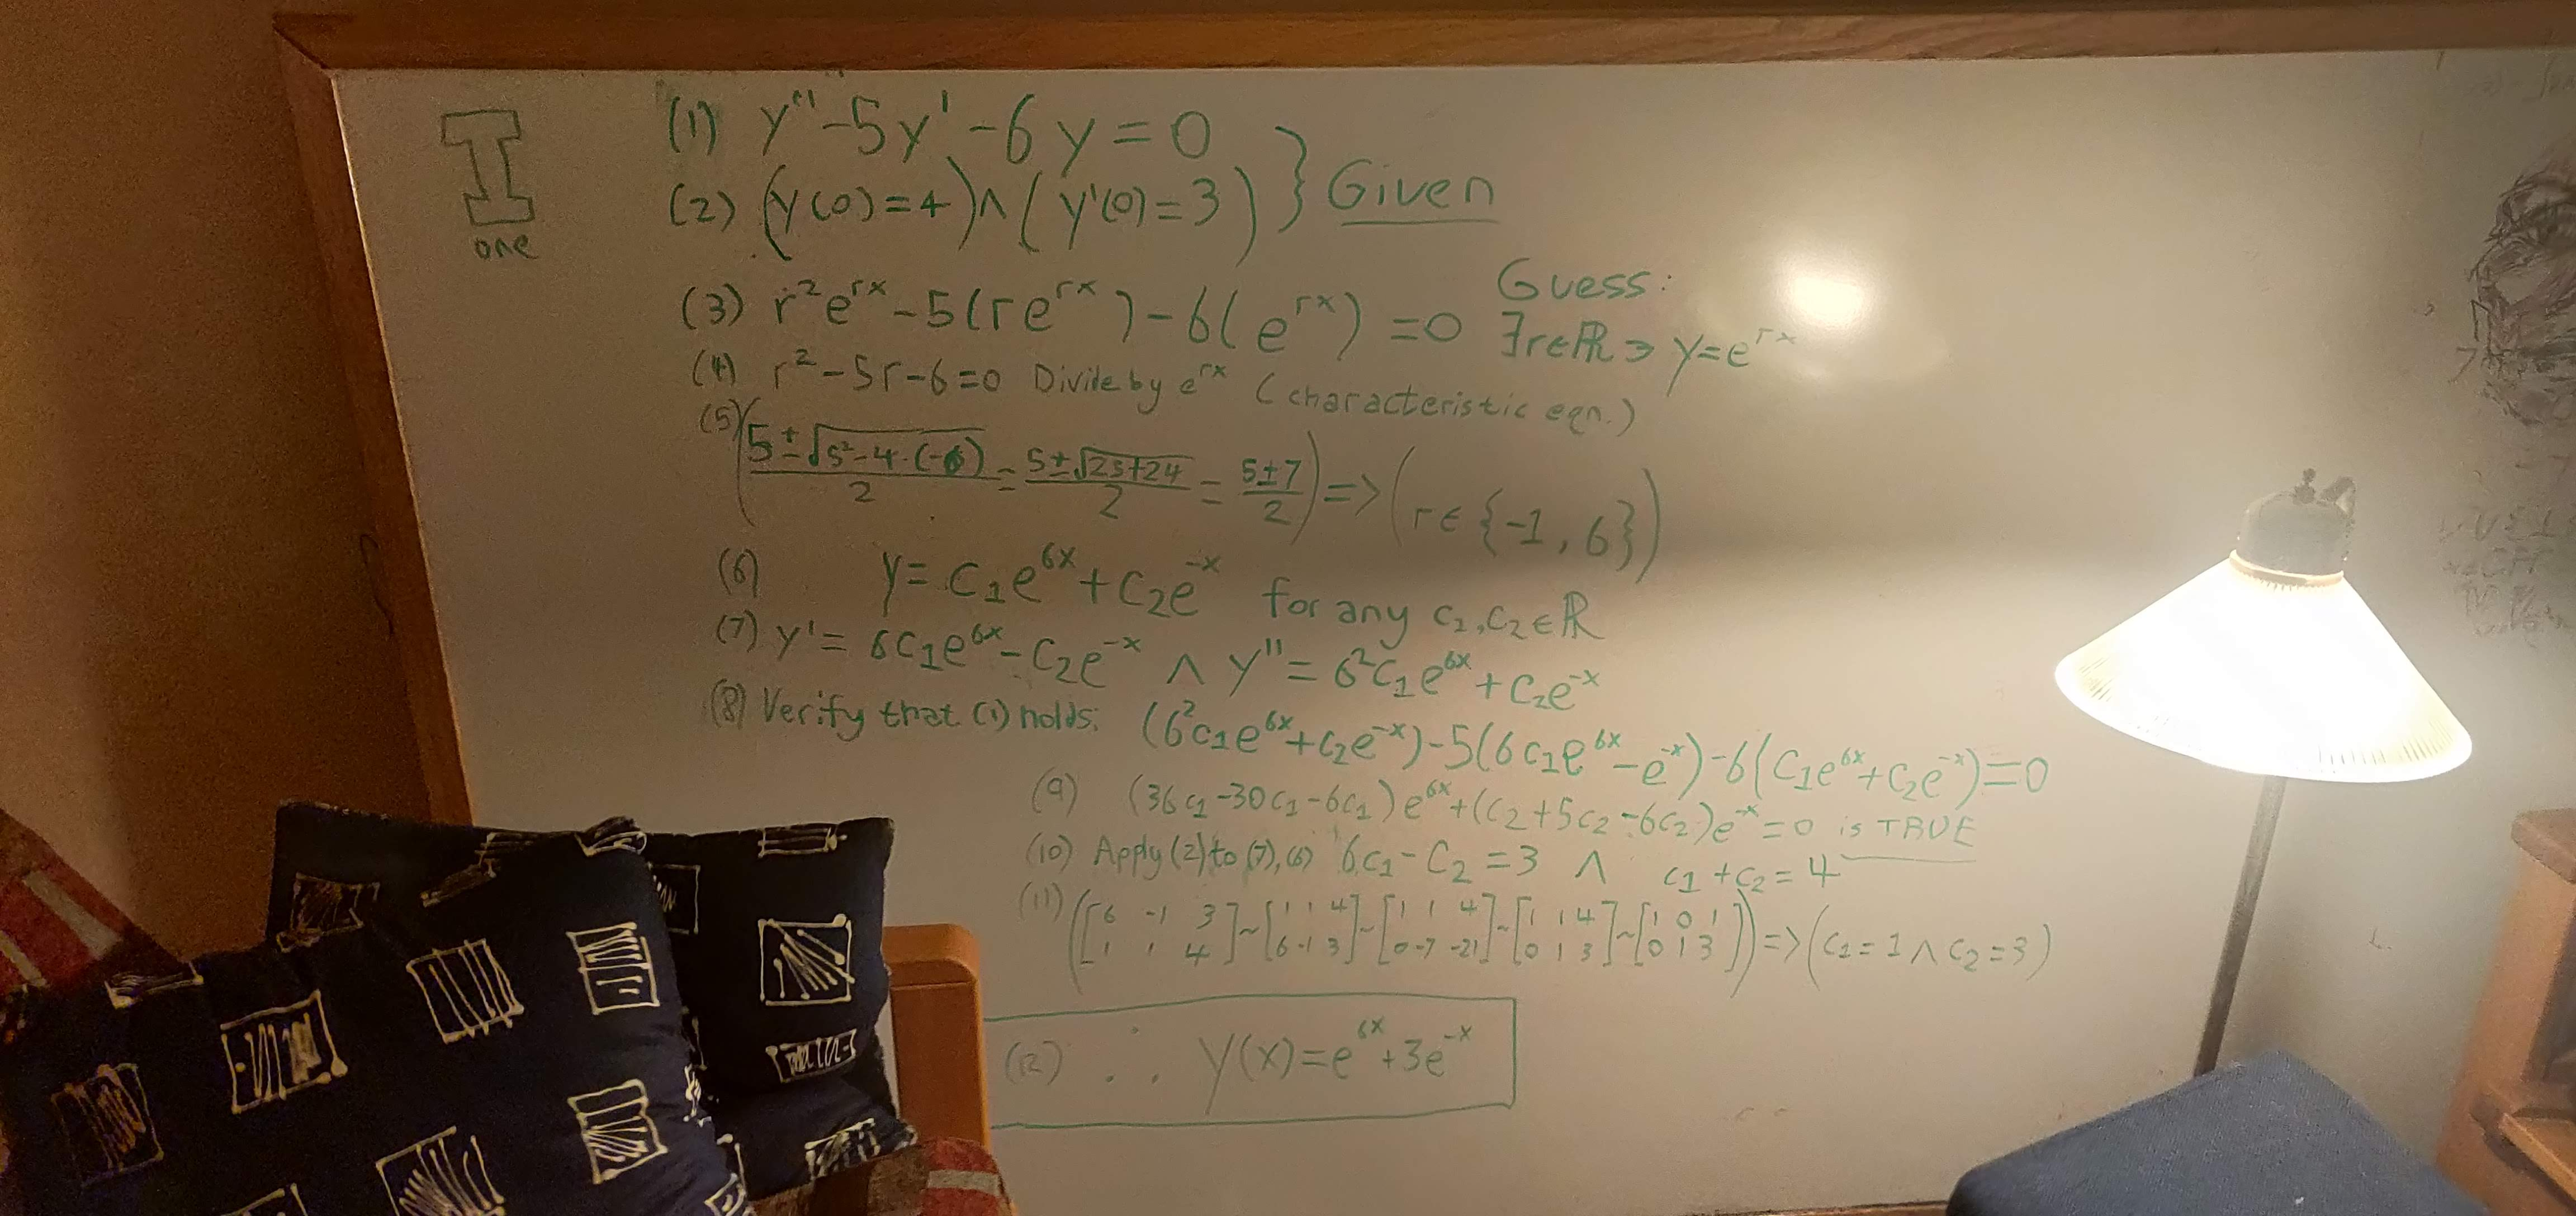
\includegraphics[scale=0.075]{1.jpg}

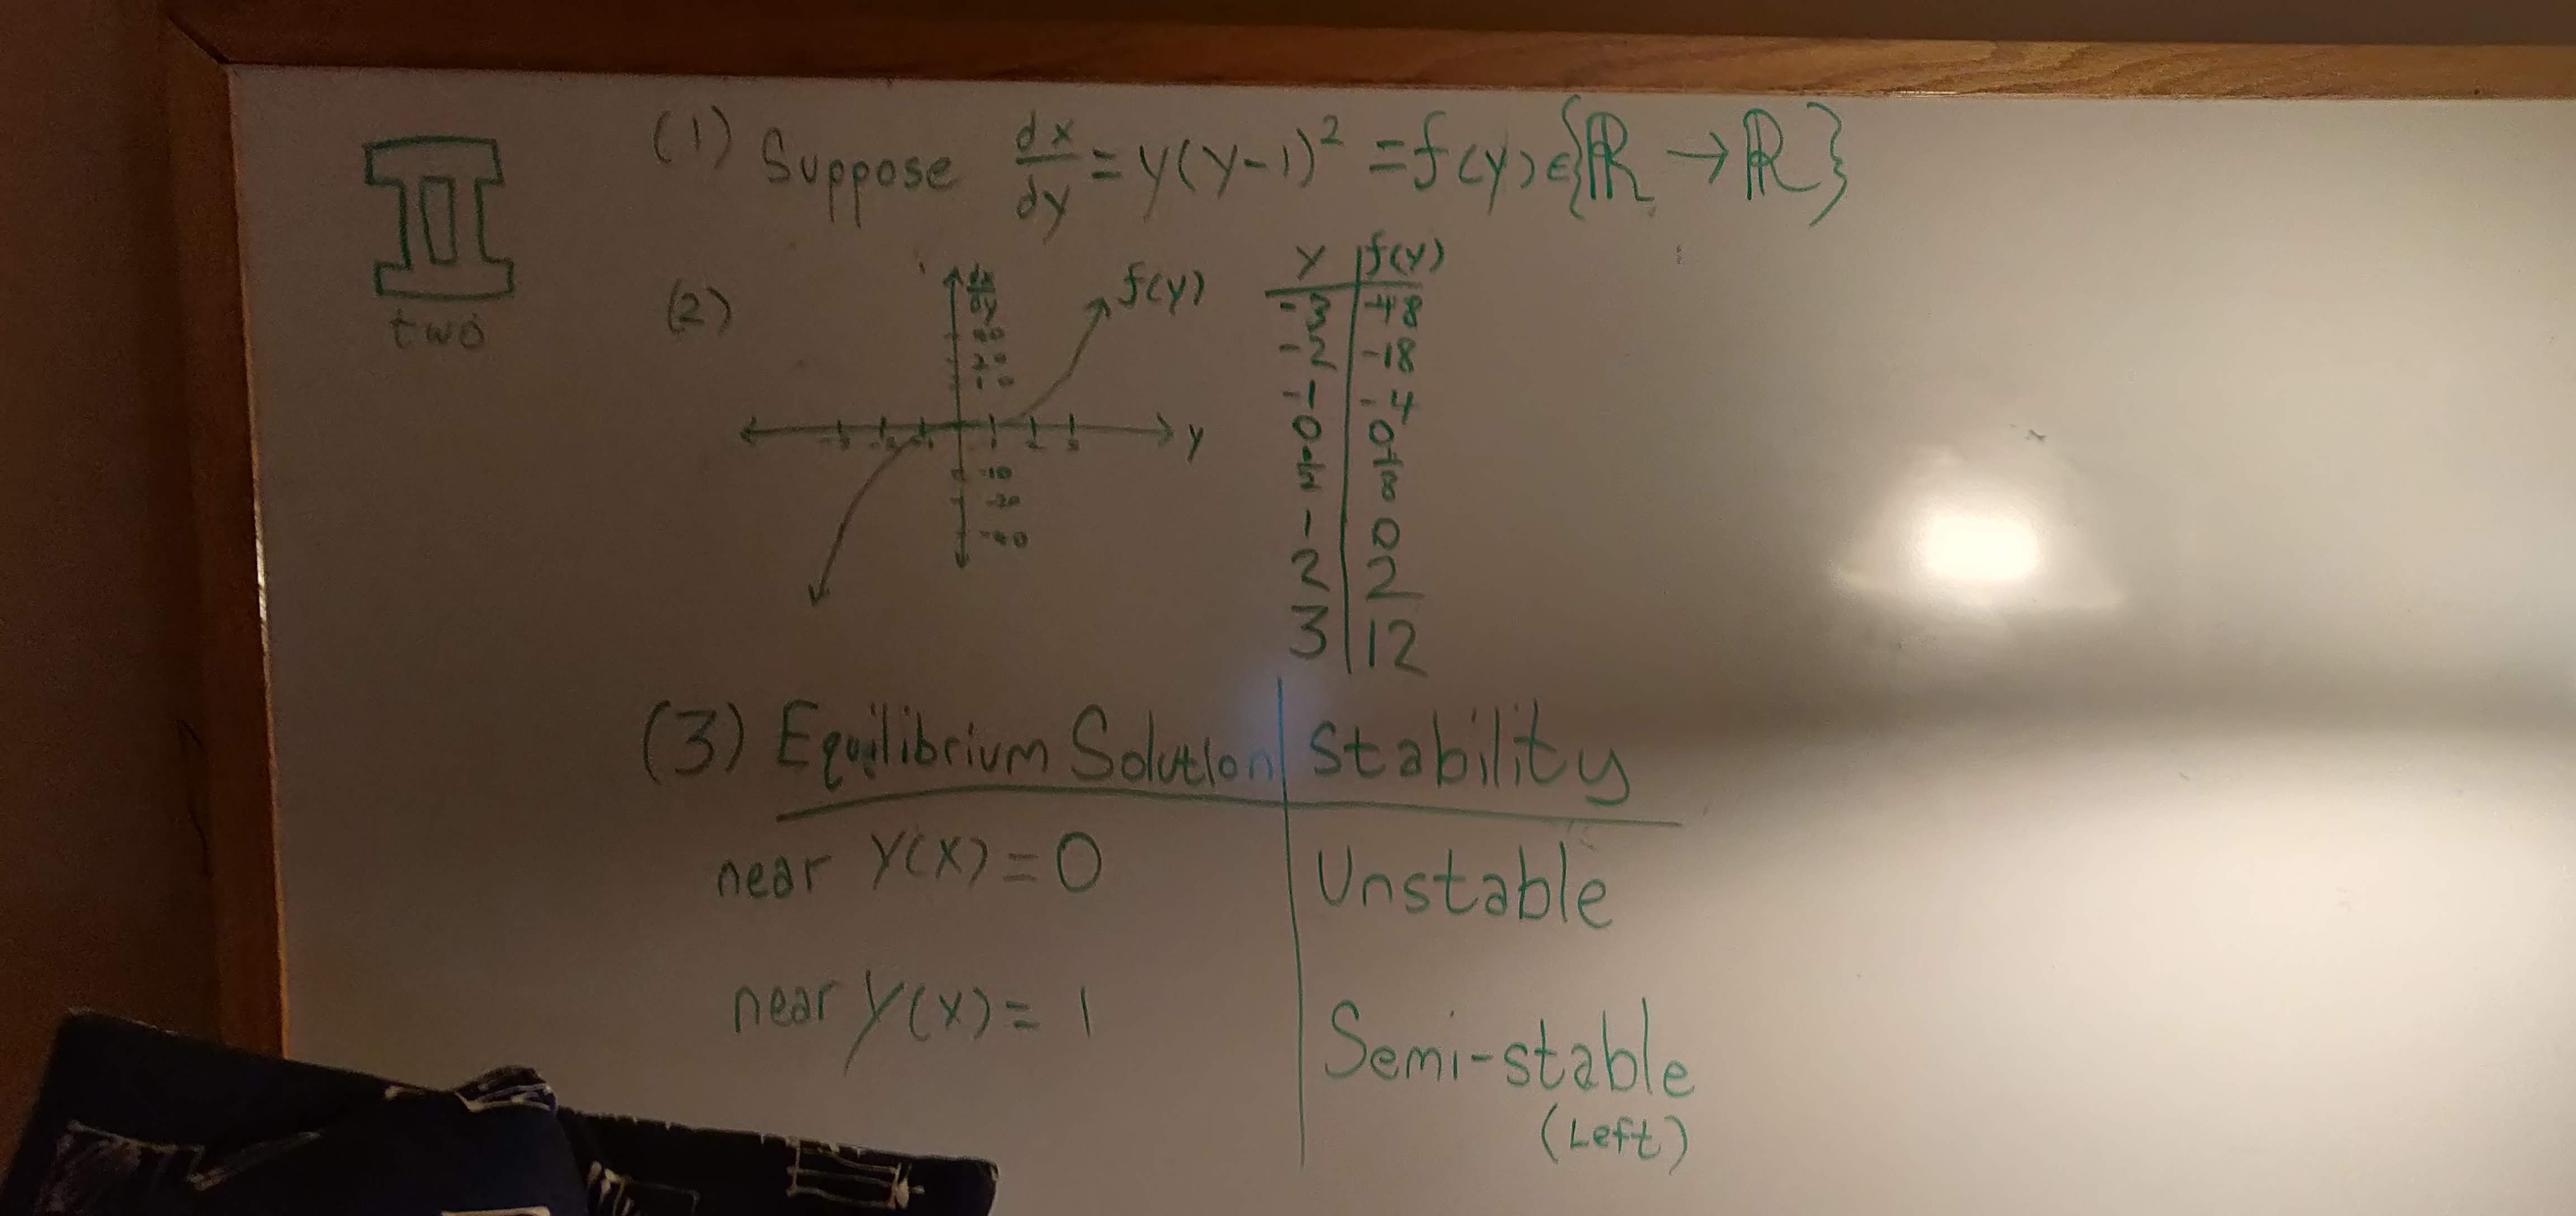
\includegraphics[scale=0.075]{2.jpg}

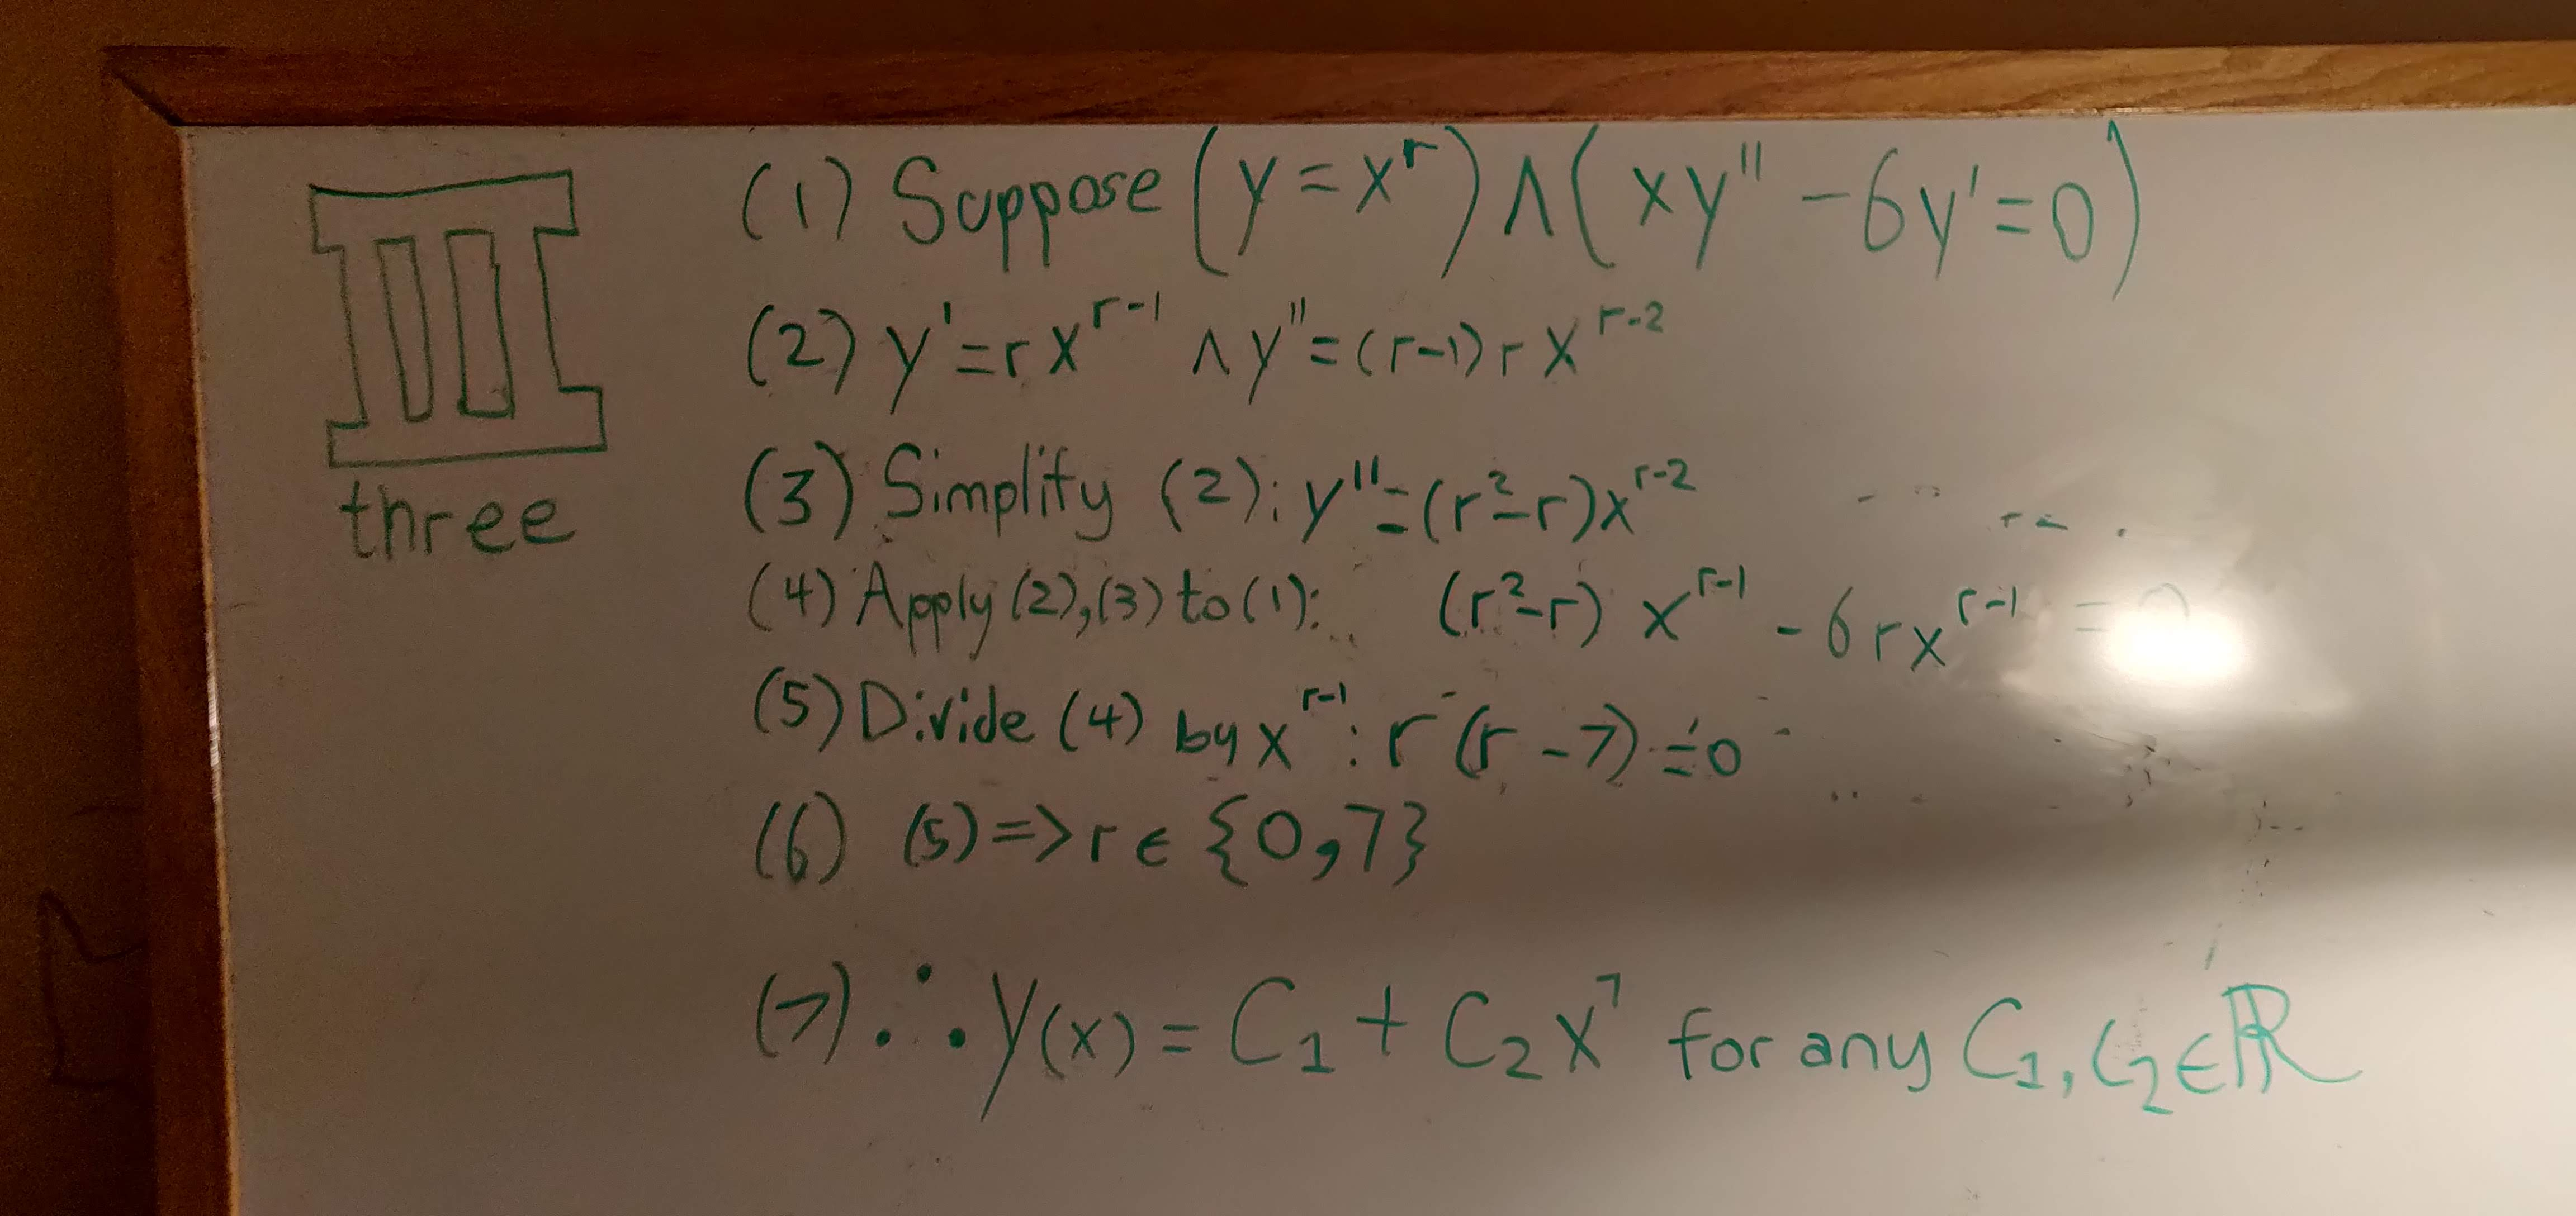
\includegraphics[scale=0.075]{3.jpg}

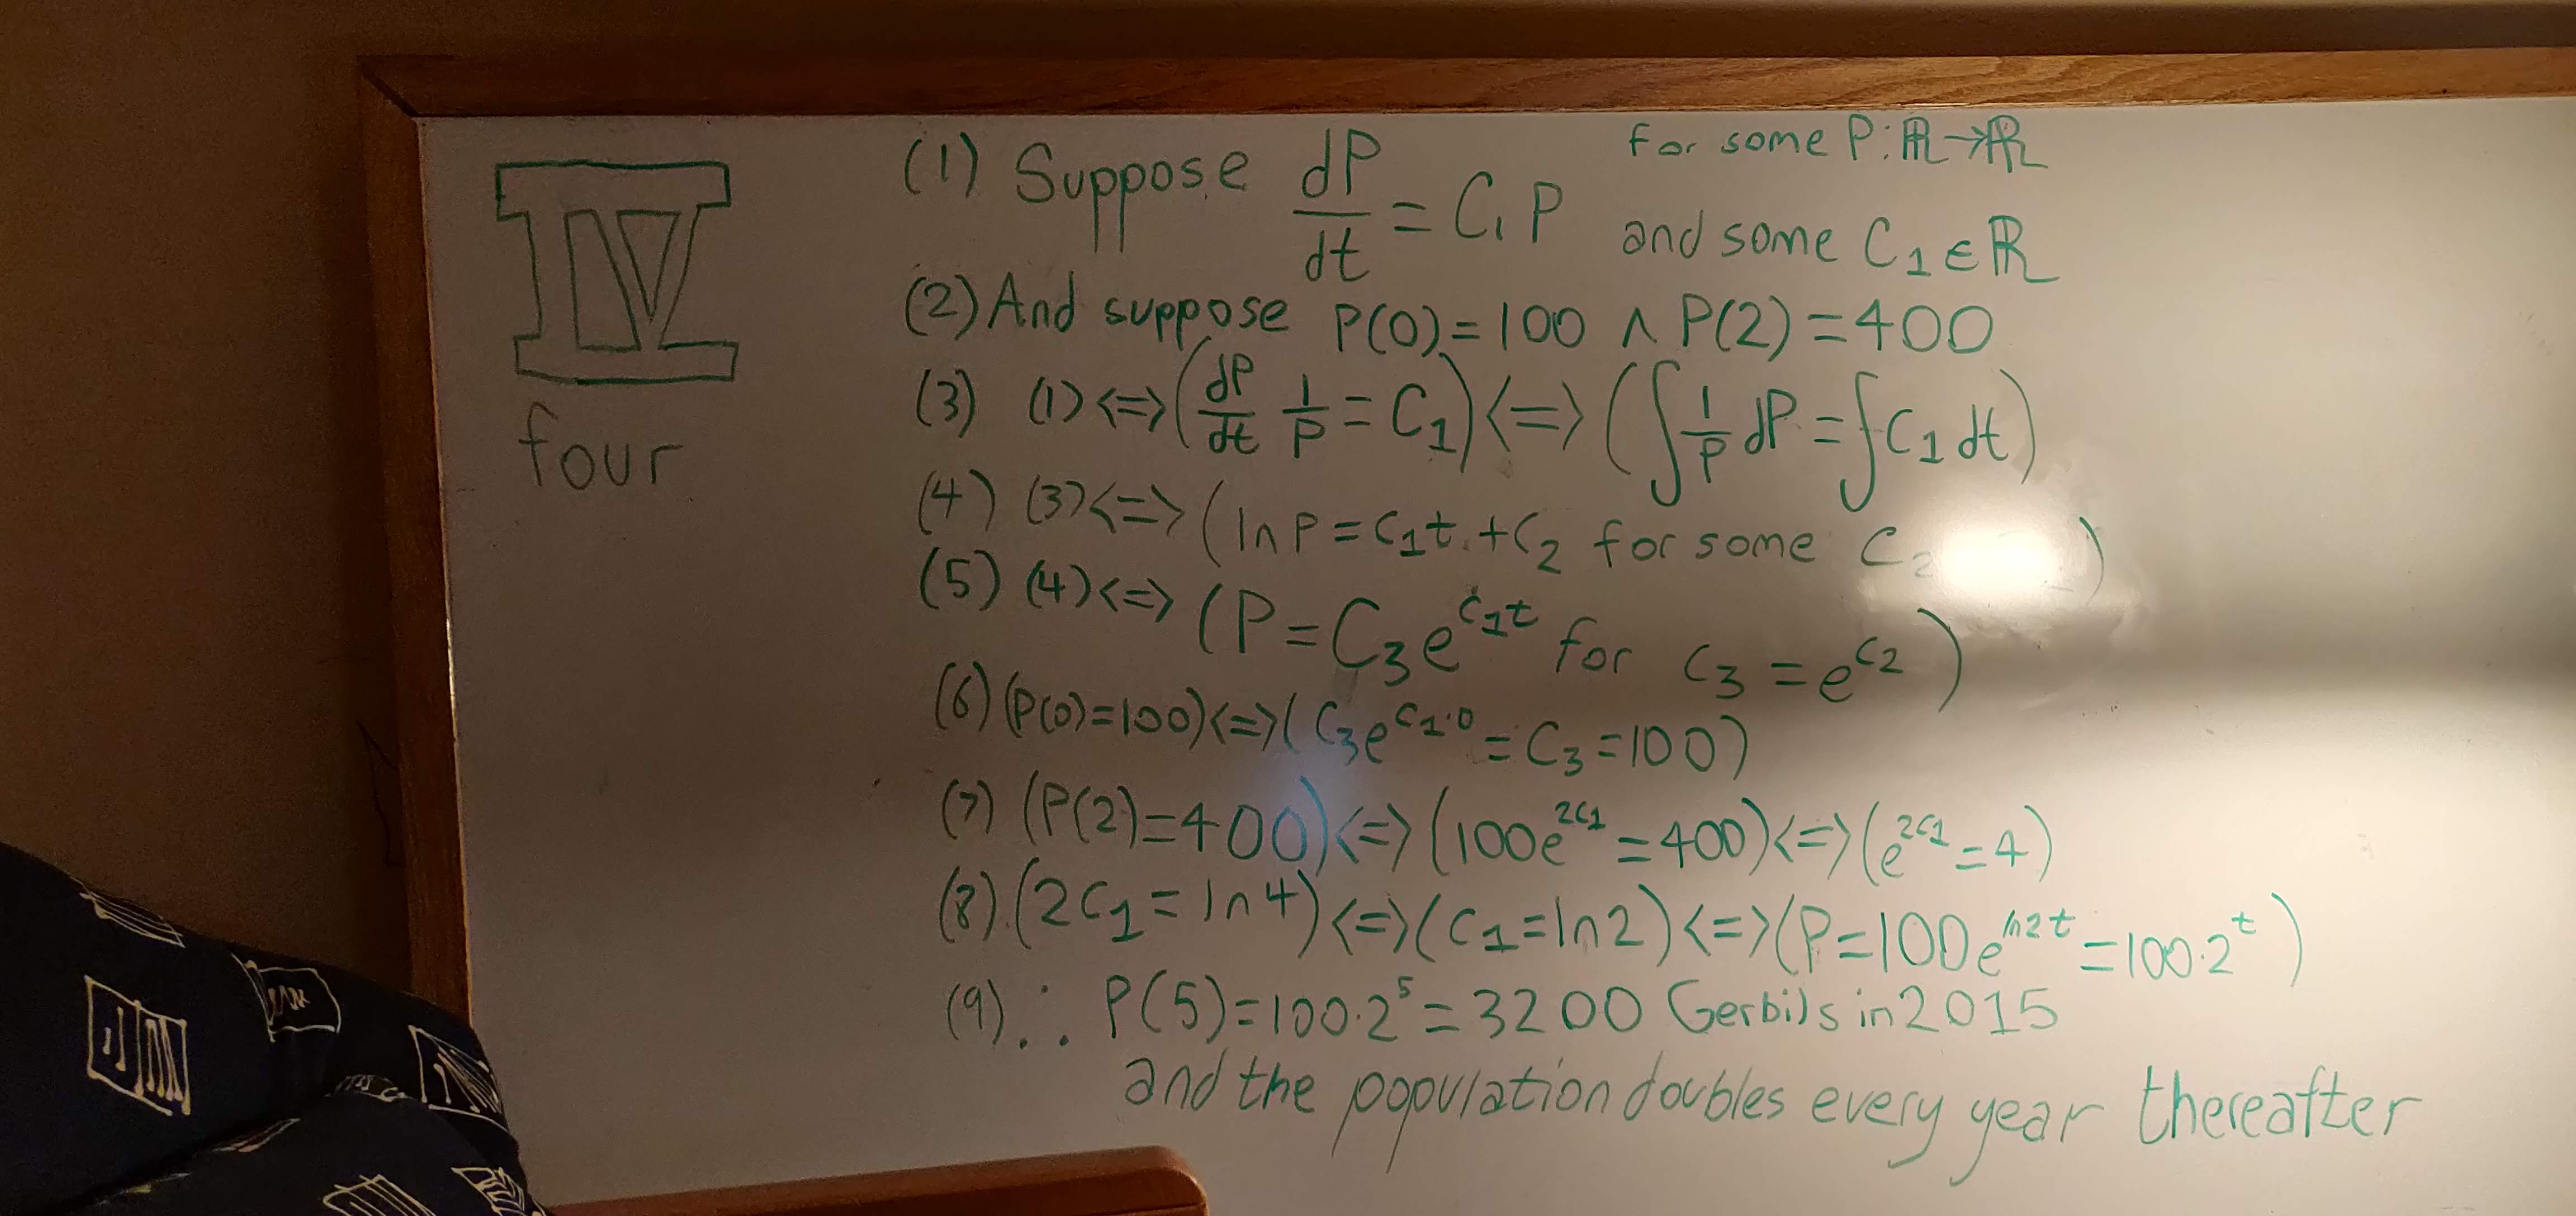
\includegraphics[scale=0.075]{4.jpg}

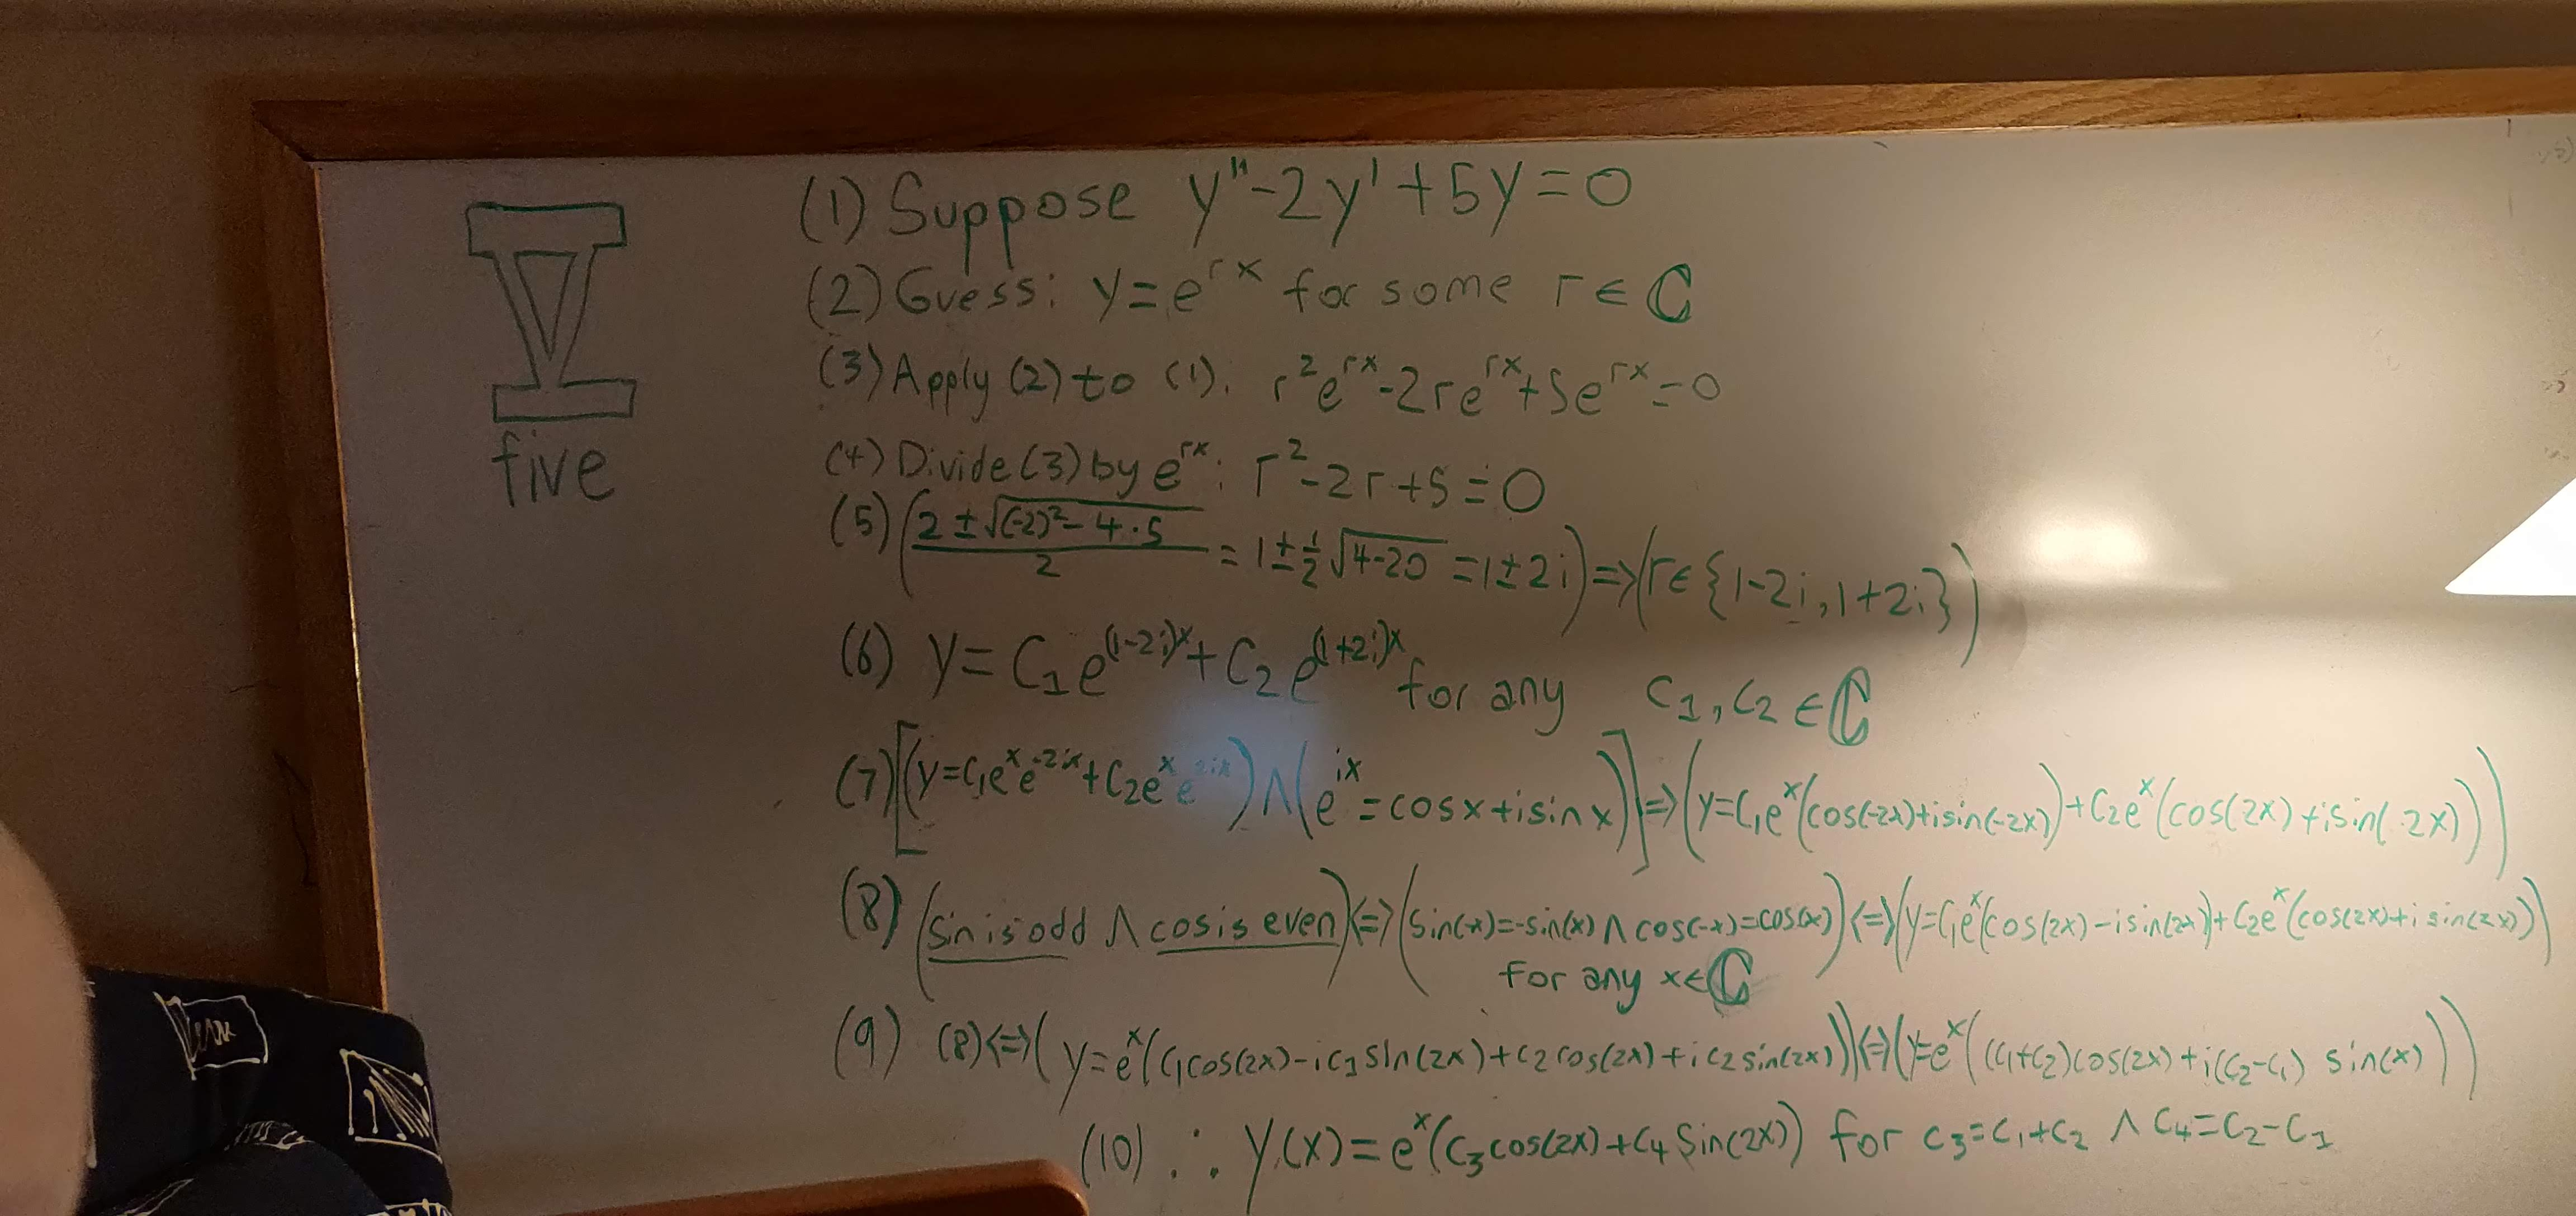
\includegraphics[scale=0.075]{5.jpg}

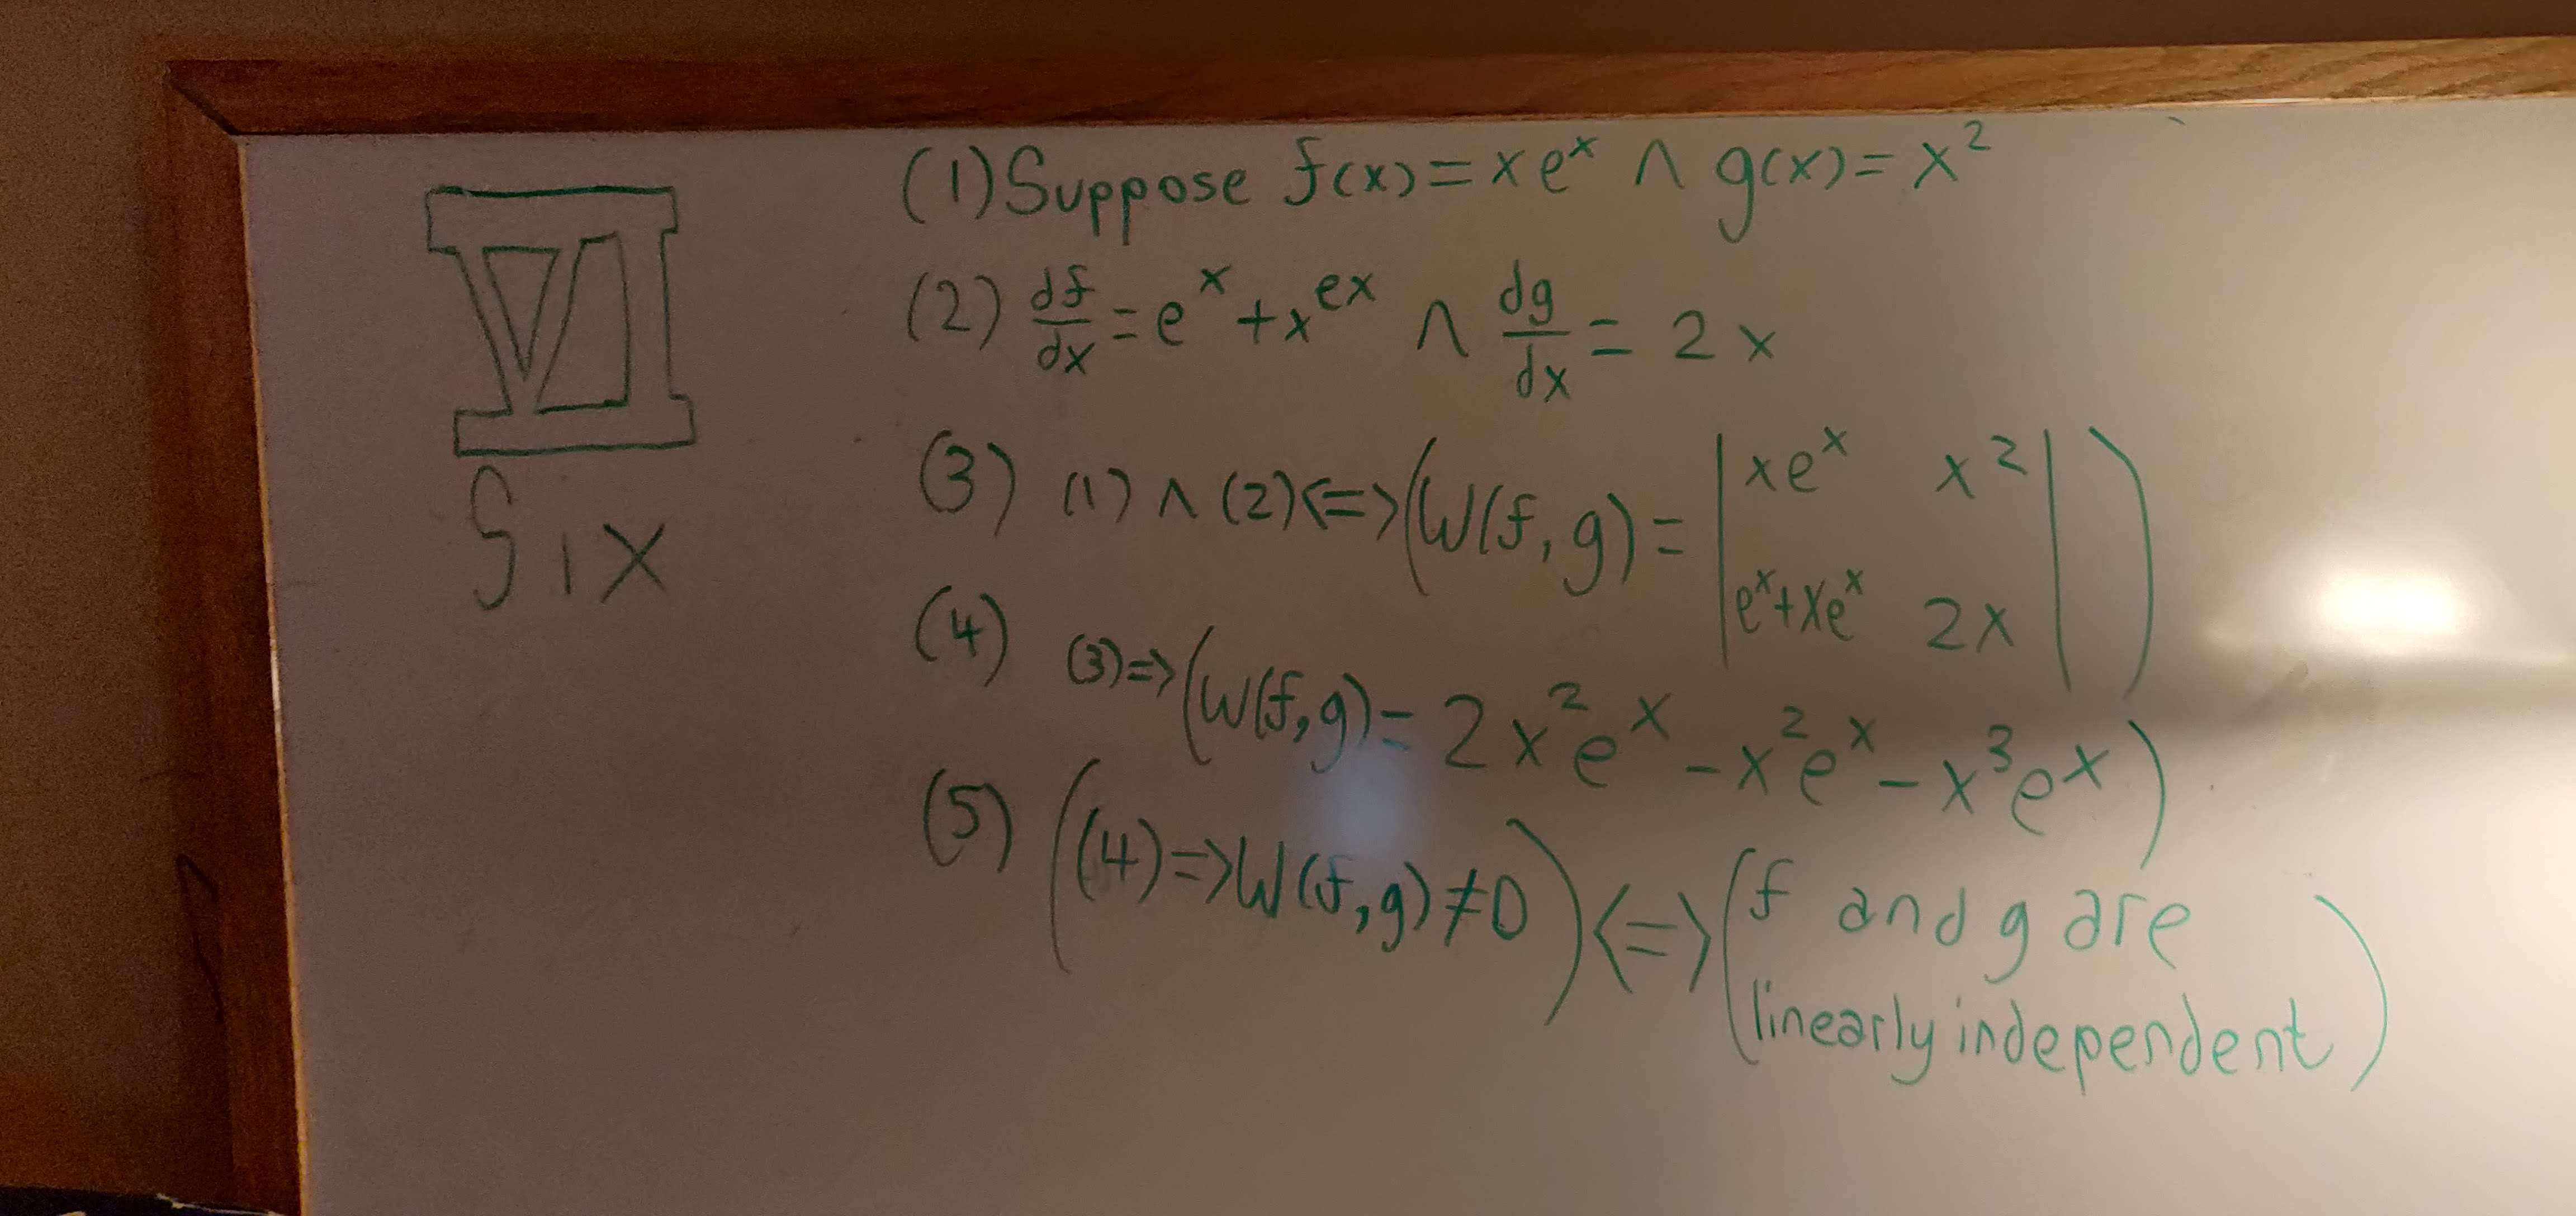
\includegraphics[scale=0.075]{6.jpg}

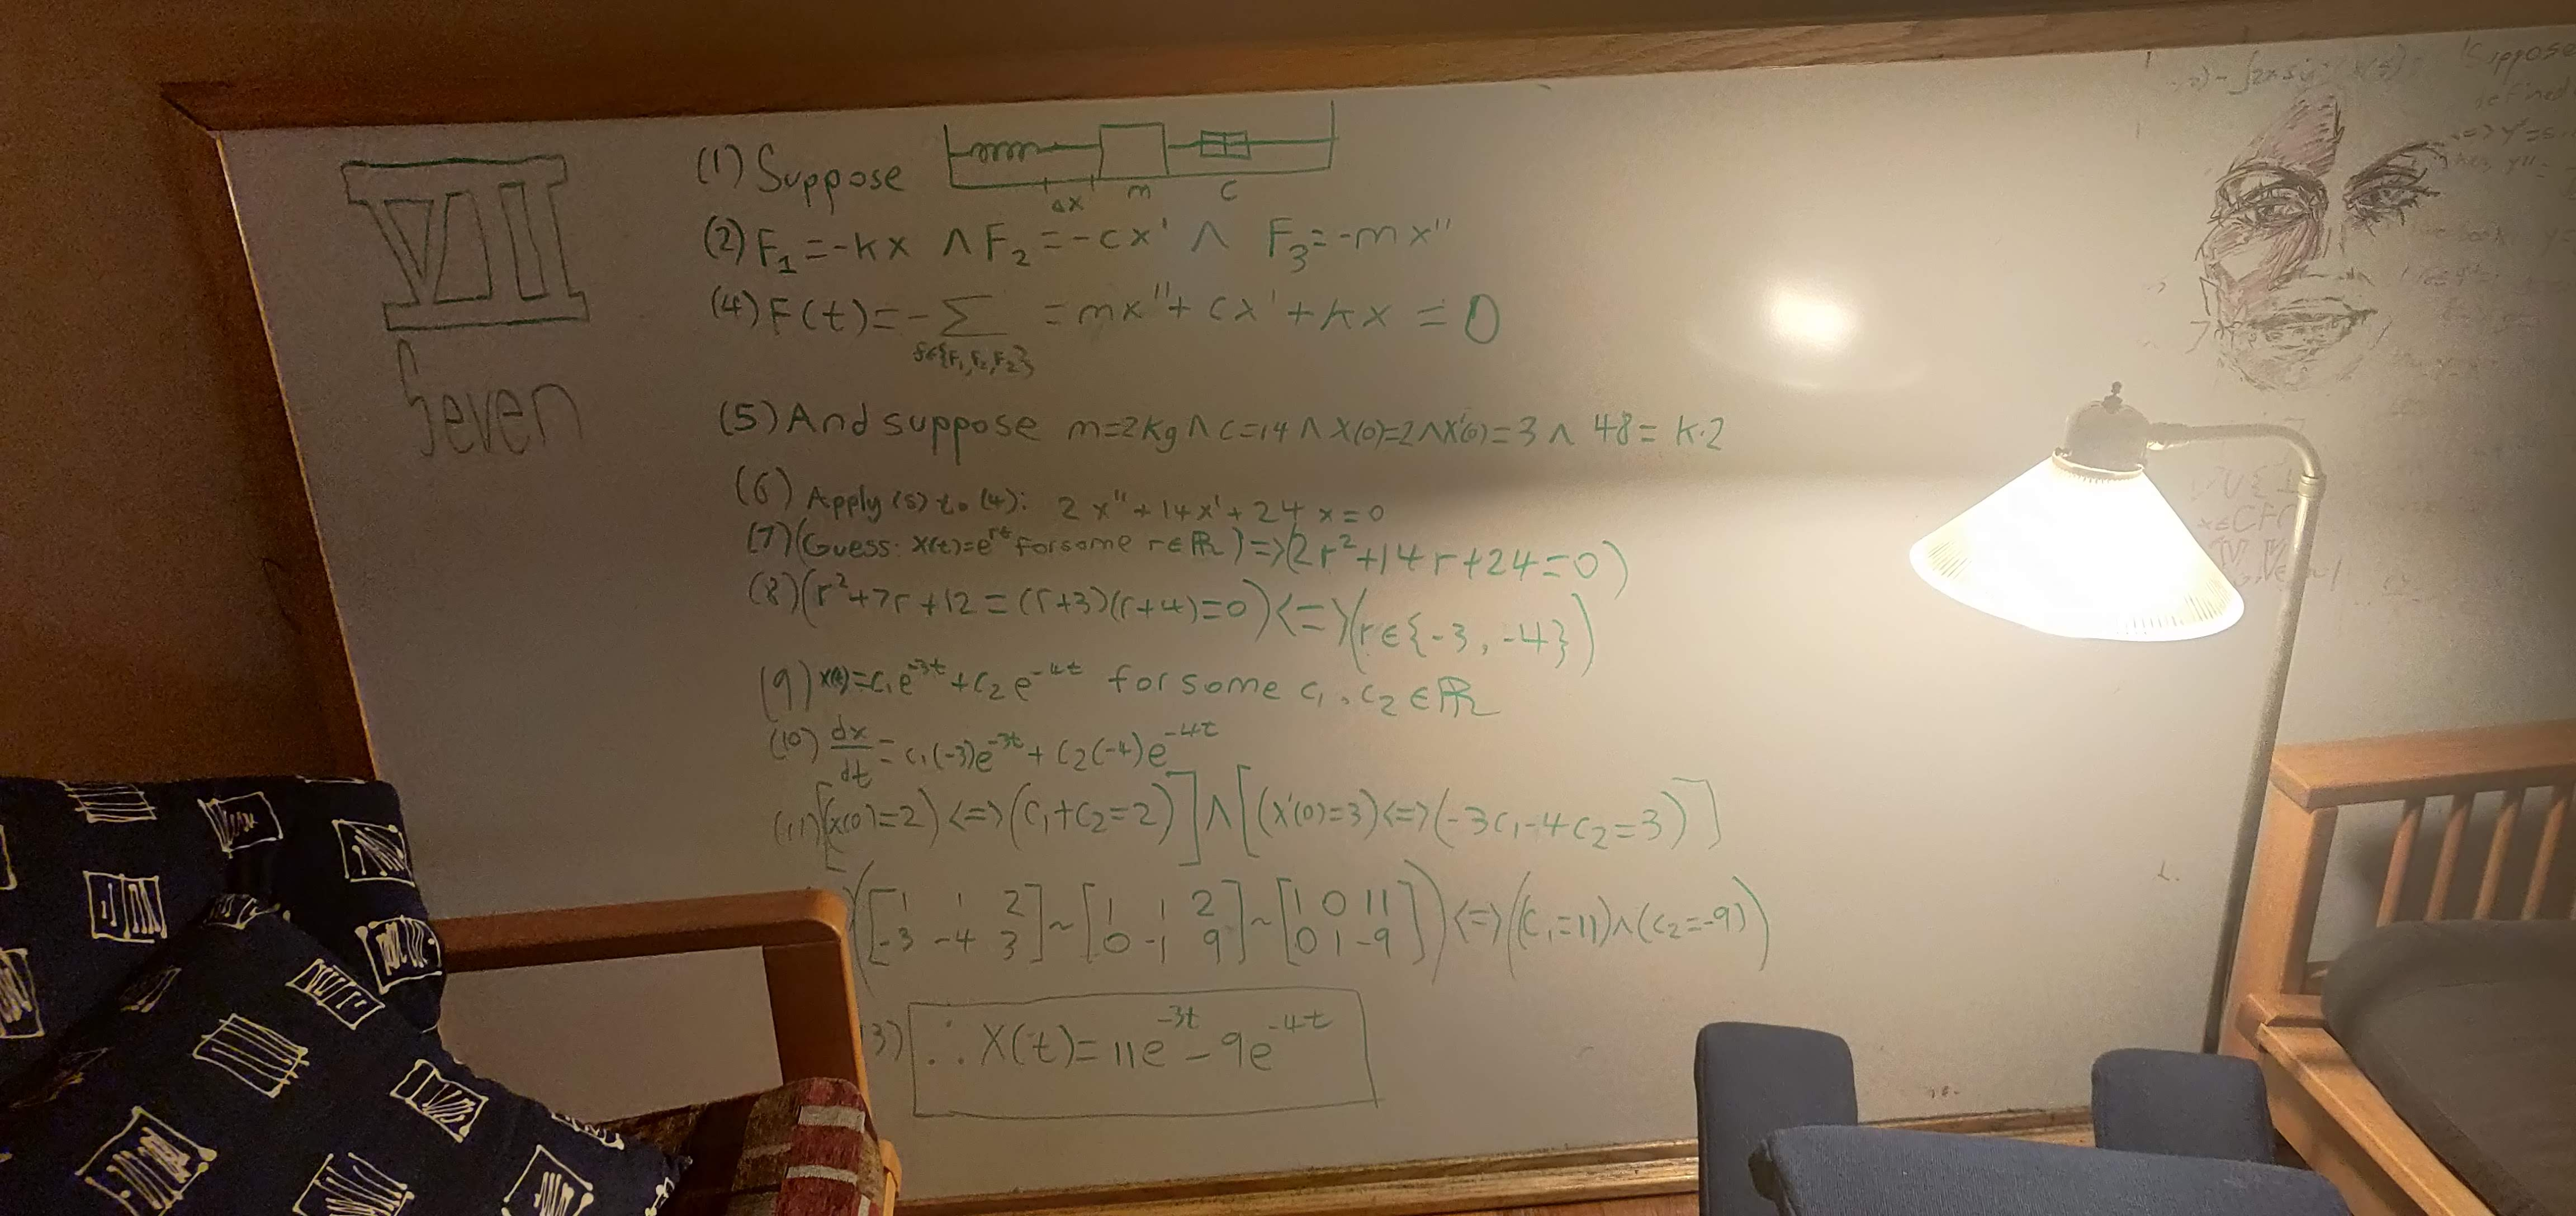
\includegraphics[scale=0.075]{7.jpg}

\medskip

\medskip

\textbf{Closing Remarks}

This concludes my submission for Exam II.
What did you think of the formatting?

The source code, the individual photos of my scratch work,
and conversations about why everyone should
typeset their work in \LaTeX\; are available on request.

\end{document}
